\begin{section}{Busqueda local}
		\begin{subsection}{Explicación}
			La heurística de busqueda local actua a partir de una solución inicial $S$, en este caso, a partir de la solución dada por la heurística constructiva. El algoritmo busca en la vecindad de la solución dada, $N(S)$, una solución mejor que ésta. Si no encuentra ninguna mejor, nos encontramos en un óptimo local (de la vecindad) que tomamos como solución del algoritmo.
						
			Decidimos revisar toda la vecindad $N(S)$ en cada iteración y quedarnos con el vecino máximo. De esta manera llegamos al optimo local por la 'máxima pendiente'. La otra opción era quedarse con el primer vecino que es mayor que el actual, pero la complejidad es la misma y creemos que revisar todos da mejores resultados.
			
			La vecindad $N(S)$ que elegimos en este problema es el conjunto de soluciones tales que no tienen uno y sólo uno de los vértices pertenecientes a $S$, es decir, $S \setminus \{v\} \cup L$ donde $L$ es un conjunto de vértices tal que $u \in L \Longleftrightarrow S \setminus \{v\} \cup \{u\}$ forma un completo.

			Para revisar la vecindad, sacamos un vértice de la solución óptima actual e intentamos agregar los vértices que no pertenecen a la clique. Luego, comparamos el tamaño de la clique que logramos contruir de esta manera con el tamaño de la clique correspondiente a la mejor solución vista de la vecindad. Si esta nueva solución es mejor, es decir, el tamaño de la clique es mayor al tamaño de la actual (mejor de la vecindad), dicha solución pasa a ser la mejor de la vecindad. Una vez revisada toda la vecindad comparamos la mejor solución encontrada en dicha vecindad con la mejor solución encontrada hasta el momento. Si es mejor, actualizamos el óptimo actual.(Figura \ref{fig:seguimiento_busqueda_local})

			% --- Figura seguimiento algoritmo constructivo ---
			\begin{figure}[H]
				\centering
		    	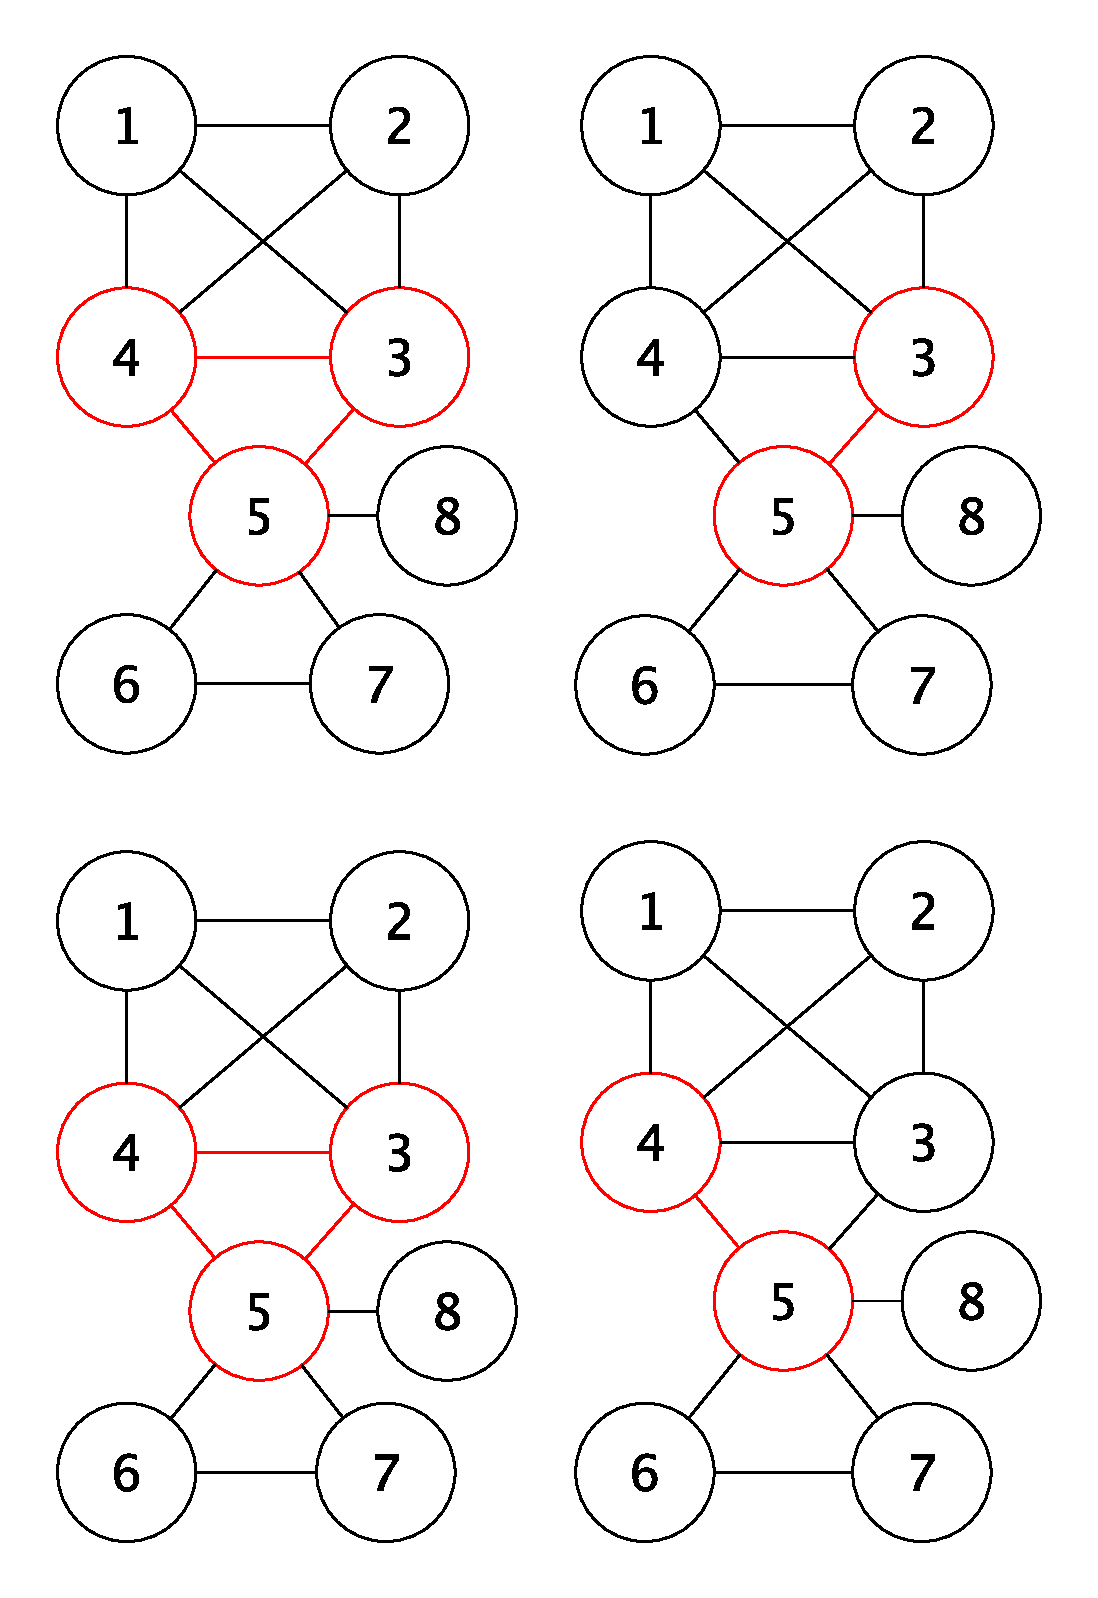
\includegraphics[scale=0.5]{busqueda_local/seguimiento.eps}
			    \caption{Ejemplo de la heurística de búsqueda local}
			    \label{fig:seguimiento_busqueda_local}
			\end{figure}
		\end{subsection}
		\begin{subsection}{Detalles de la implementación}
			Almacenamos las relaciones entre los vértices en una matriz de $n \times n$, donde $n$ es la cantidad de vértices. Cada posición $(i,j)$ de la matriz contiene un $uno$ si existe la arista $(i,j)$ y un $cero$ en caso contrario. De esta forma se le asigna un número a cada vértice.\VSP

			A continuación, se muestra el pseudocódigo de la heurística de búsqueda local.\\

			Sea $n$ la cantidad de vértices del grafo.

			\begin{pseudo}
				\func{busqueda\_local}{solucion,tamanyo,matriz\_adyacencia}
				\tab $\IF tamanyo==1 \OR tamanyo==n$\\
				\tab \tab $\RET tamanyo$\\
				\tab $grados[n] \leftarrow ordenar\_grados(matriz\_adyacencia)$\\
				\tab $inicializar\_estructuras$\\
				\tab $\WHILE mejore$\\
				\tab \tab $\FOR i \TO n$\\
				\tab \tab \tab $sacar\_de\_clique(actual,i)$\\
				\tab \tab \tab $agrandar\_clique(actual,matriz\_adyacencia)$\\
				\tab \tab \tab$\IF tam\_actual>tam\_mejor\_vecindad$\\
				\tab \tab \tab \tab $actualizar\_mejor\_vecindad$\\
				\tab \tab \tab$\ELSE$\\
				\tab \tab \tab \tab $reconstruir(actual)$\\
				\tab \tab \IF $tam\_mejor\_vecindad>tamanyo$\\
				\tab \tab \tab $mejore 	\leftarrow true$\\
				\tab \tab \tab $actualizar\_solucion$\\
				\tab \RET $tamanyo$\\
			\end{pseudo}

		La primer cláusula \texttt{if} verifica si la solución constructiva encontró la clique tanto completa como la de un elemento. En ambos casos no tiene sentido aplicar la búsqueda local ya que, si encontró el completo, esta solución no podrá ser mejorada, al contener todos los vértices. Si sólo encontró un vértice, implica que el de grado mayor en el grafo es de grado cero, por lo tanto, todos sus vértices son de grado cero. 

		\begin{itemize}
			\item \texttt{inicializar\_estructuras:} Consiste en hacer dos copias de la solución, una para mejor vecindad y otra para actual, y setear dos variables que representan el tamaño de la clique de cada uno de los arreglos.
		
			\item \texttt{sacar\_de\_clique:} Esta función setea en $falso$ la posición $i$ del arreglo $actual$, es decir, excluye el vértice $i$ de la solución actual. Además, decrementa el tamaño de la clique, variable $tam\_actual$ y resetea una variable $nodo$ que indica si despues logra agregar algún vértice, esto sirve para reconstruir la solución en caso de ser necesario (conseguir un tamaño de clique igual al tamaño de la clique desde la que partió).

			\item \texttt{agrandar\_clique:} Esta función se encarga de buscar entre los vértices que actualmente no pertenecen a la clique e intenta agregarlos (agrega todo vértice que forma un completo con los ya pertenecientes), con el objeto de conseguir una de mayor tamaño. Por otro lado, setea $nodo$ con el valor del último vértice que agrega.

			\item \texttt{reconstruir:} En el caso donde el tamaño de la clique que logro contruir es igual al tamaño de la clique inicial, como queremos obtener el mejor de la vecindad, reconstruimos la clique anterior y continuamos, es decir, eliminamos $nodo$ y volvemos a agregar $i$.
			
			\item \texttt{actualizar\_mejor\_vecindad y actualizar\_solucion:} al encontrar una solución que es mejor a la que el algoritmo posee hasta ese momento, dependiendo del caso, la salva en uno de estos dos arreglos ($mejor\_vecindad$ o $actual$).
			
		\end{itemize}
		\end{subsection}
		\begin{subsection}{Desventajas}
		
		El algoritmo es estrictamente dependiente de la numeración inicial de los vértices. Para vértices de igual grado, al ordenarlos tiene prioridad el de menor numeración.(Figura \ref{fig:seguimiento_caso_malo_busqueda_local})

			% --- Figura seguimiento algoritmo busqueda local ---
			\begin{figure}[H]
				\centering
		    	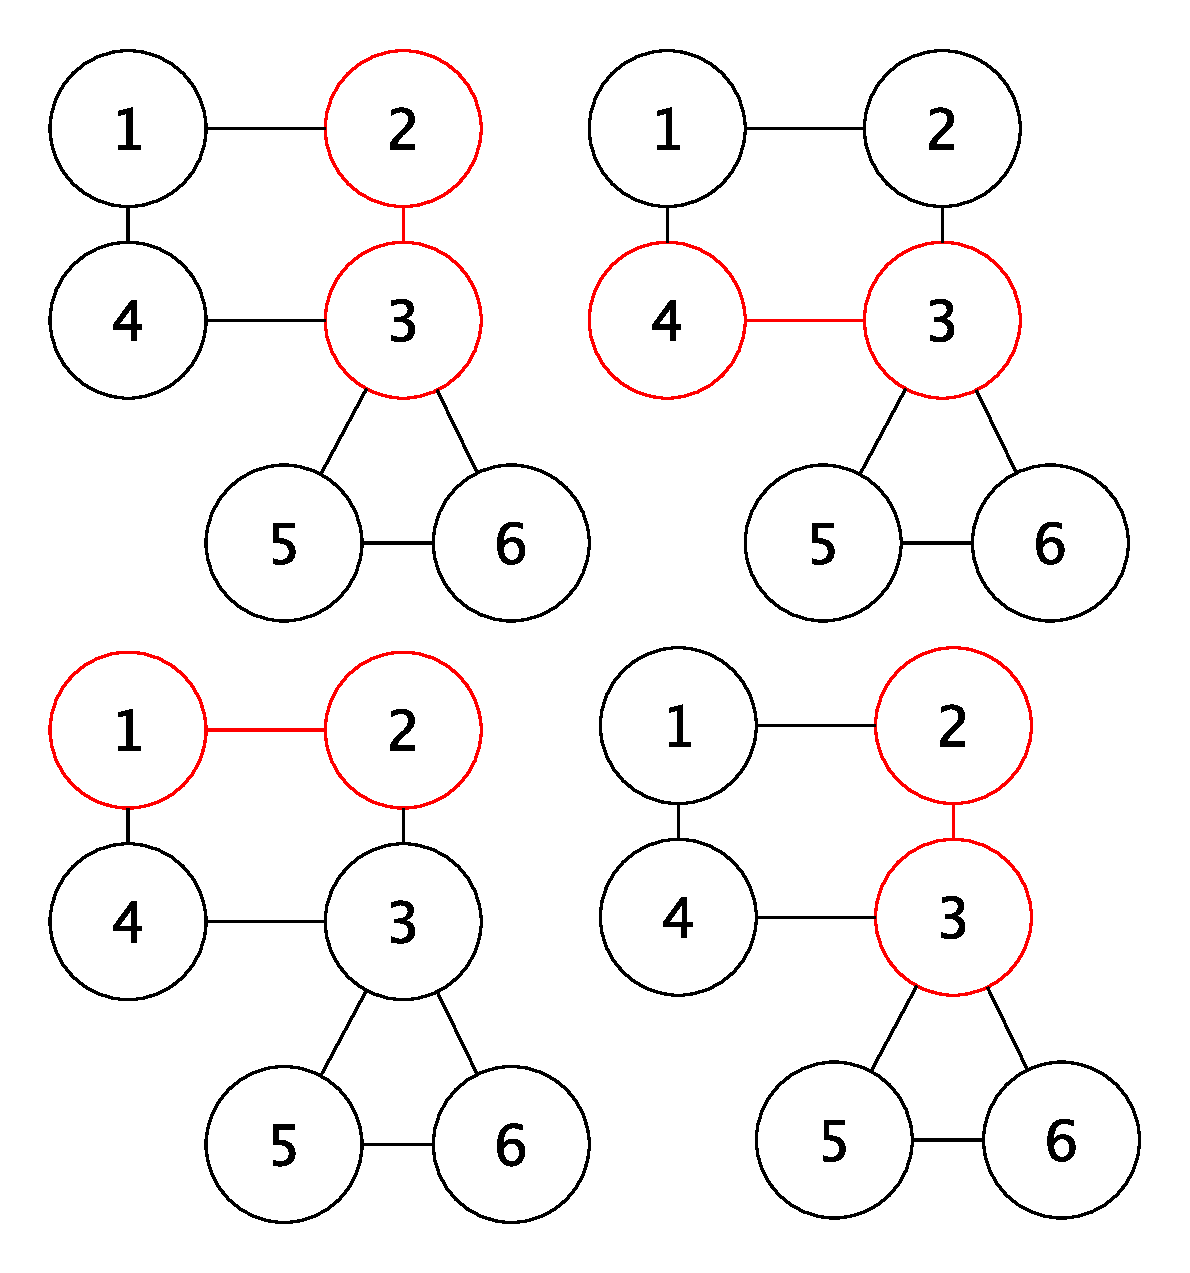
\includegraphics[scale=0.5]{busqueda_local/segCasoMalo.eps}
			    \caption{Caso malo para la heurística de búsqueda local}
			    \label{fig:seguimiento_caso_malo_busqueda_local}
			\end{figure}


		La clique dada por la heurística constructiva es el $<2,3>$.
		Cuando el algoritmo (búsqueda local) saca el vértice $dos$ de la clique, se mueve a la clique $<3,4>$ ya que todos sus adyacentes tienen grado dos y el $cuatro$ es el de menor numeración (excluyendo el $dos$ que es el que acaba de sacar). Como no logra mejorar (no encuentra una clique que posea al $tres$, al $cuatro$, y además algún otro vértice), no actualiza el mejor de la vecindad quedando el $<2,3>$. Prueba entonces sacando el $tres$, sin poder mejorar. Por lo tanto, la solución final es la que viene dada por el algortimo constructivo.

		(Figura \ref{fig:seguimiento_caso_malo_busqueda_local2})

			% --- Figura seguimiento algoritmo busqueda local ---
			\begin{figure}[H]
				\centering
		    	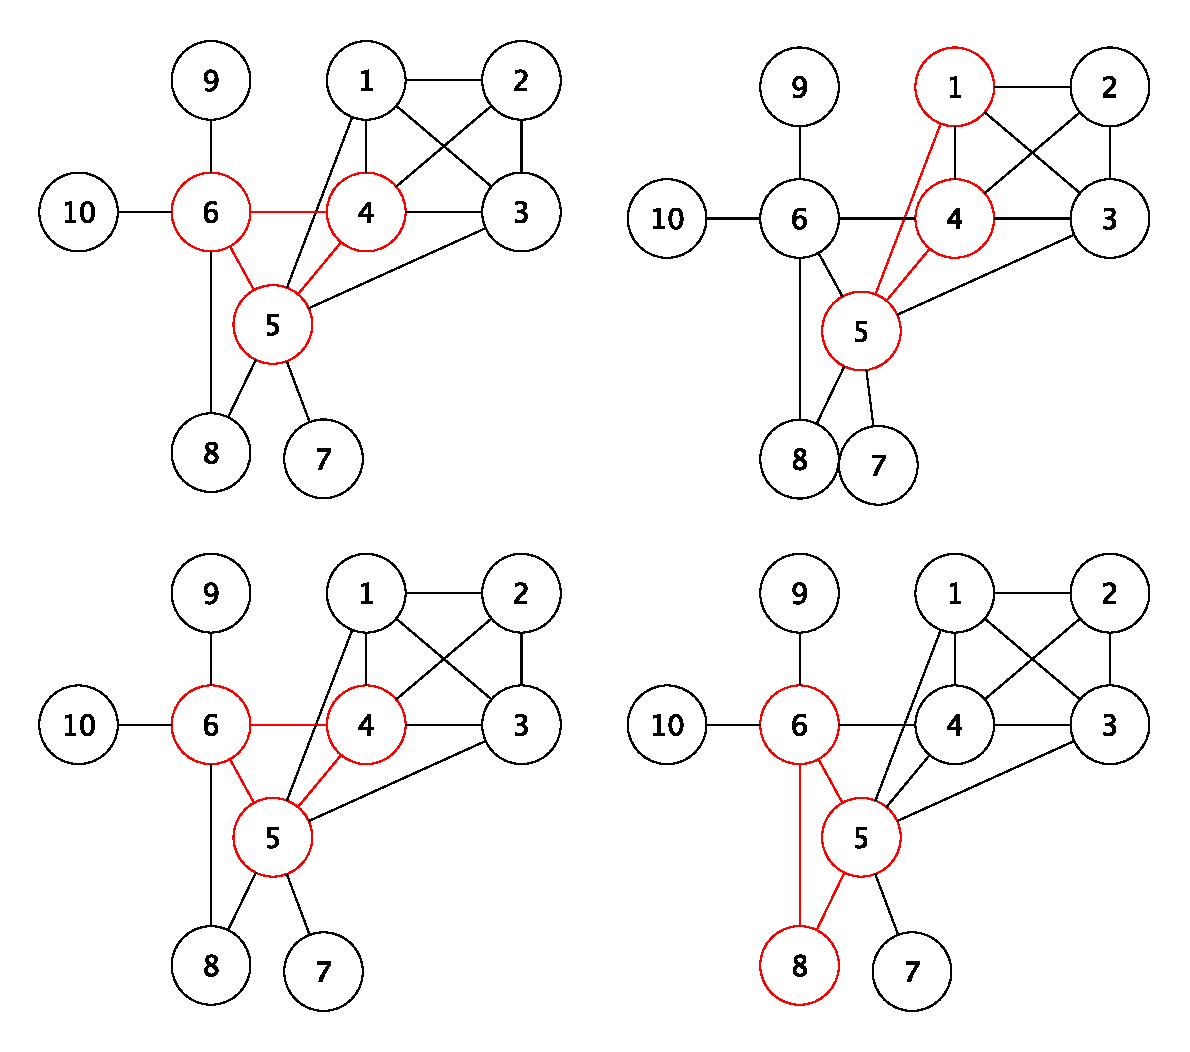
\includegraphics[scale=0.5]{busqueda_local/segCasoMalo2.eps}
			    \caption{Caso malo para la heurística de búsqueda local}
			    \label{fig:seguimiento_caso_malo_busqueda_local2}
			\end{figure}

		ACAAAA ACAAAA ESCRIBI
		\end{subsection}
		\begin{subsection}{Complejidad temporal}
			En un pricipio el algoritmo inicializa el arreglo de los $grados$ y lo ordena aplicando QuickSort, lo que tiene un costo de $n^2$. Luego, obtiene la solución inicial mediante la heurística constructiva que como ya vimos tiene también un costo de $n^2$ e inicializa los arreglos $actual$ y $mejor\_vecindad$ con costo lineal.

			La función $sacar\_de\_clique$ y $reconstruir$ tienen costo constante ya que consta sólo de indexaciones, asignaciones y otras operaciones elementales.

			La función $agrandar\_clique$ tiene costo $n^2$ porque recorre todos los vértices y para cada uno de los que todavía no pertenece a la clique, verifica si puede agregarlo. Para esto, recorre nuevamente todos los vértices y corrobora que sea adyacente a cada uno de los pertenecientes a la clique.

			La complejidad final del algoritmo es $n^4$ porque el ciclo \texttt{while} itera a lo sumo $n$ veces (la solución final puede verse mejorada a lo sumo $n$ veces, ver observación) y por cada una de estas el ciclo \texttt{for} itera exactamente $n$ veces. En cada iteración del \texttt{for} hay una llamada a la función $sacar\_de\_clique$ y $agrandar\_clique$ las cuales tienen un costo de $n^2$. Eventualmente hay una llamada a $reconstruir$ lo que no altera la complejidad, ya que su costo es constante.
			
			\texttt{Observación: } El costo lineal en función de la cantidad de vértices del ciclo \texttt{while} está acotado por el caso hipotético de comenzar por una clique trivial, y en cada iteración, aumentar la clique en uno. Esto no puede pasar ya que se trataría de un grafo completo, que el algoritmo constructivo encontraría. En ese caso, el algoritmo termina antes de la primera iteración del \texttt{while}.
		\end{subsection}
\end{section}



